\begin{center}

\includegraphics[width=0.4\textwidth]{content/3/chapter6/images/15.png}\\
Cippi在指挥着火车
\end{center}

信号量是一种同步机制,用于控制对共享资源的并发访问。计数信号量是一种特殊的信号量,其计数器的值大于零,计数器在构造函数中初始化。获取信号量会减少计数,释放信号量会增加计数器。若线程试图在计数器为零时获取信号量,则该线程将阻塞,直到另一个线程通过释放信号量来增加计数。

\begin{tcolorbox}[breakable,enhanced jigsaw,colback=blue!5!white,colframe=blue!75!black,title={Edsger W. Dijkstra发明了信号量}]
	
荷兰计算机科学家\href{https://en.wikipedia.org/wiki/Edsger_W._Dijkstra}{Edsger W. Dijkstra}在1965年提出了信号量的概念,是一种具有队列和计数器的数据结构。计数器初始化为一个等于或大于零的值,支持等待和信号两种操作,操作等待获取信号量并减少计数。若计数器为零,将阻止线程获取信号量。操作信号释放信号量并增加计数。阻塞的线程会添加到队列中以避免\href{https://en.wikipedia.org/wiki/Starvation_(computer_science)}{饥饿}。而最初,信号量是用在铁路上的。
	
\end{tcolorbox}

\begin{center}
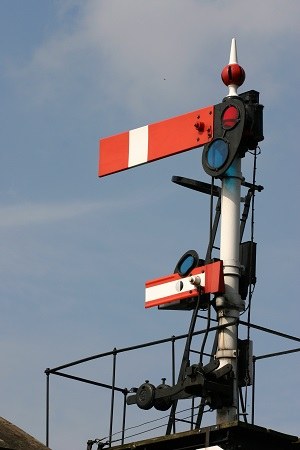
\includegraphics[width=0.35\textwidth]{content/3/chapter6/images/16.png}\\
信号量
\end{center}

相关的英文维基百科最初由AmosWolfe上传 - \href{https://commons.wikimedia.org/w/index.php?curid=1972304}{Transferred from en.wikipedia to Commons., CC BY 2.0,}

C++20支持std::binary\_semaphore,其是std::counting\_semaphore<1>的别名,最大值是1。std::binary\_semaphores可以用来实现\href{https://en.cppreference.com/w/cpp/named_req/BasicLockable}{锁}。

\begin{lstlisting}[style=styleCXX]
using binary_semaphore = std::counting_semaphore<1>;
\end{lstlisting}

与std::mutex相反,std::counting\_semaphore不绑定到线程,所以信号量调用的获取和释放可以发生在不同的线程上。下表给出了std::counting\_semaphore的接口。

\begin{table}[H]
\centering
\begin{tabular}{ll}
\textbf{成员函数} & \textbf{std::counting\_semaphore sem成员函数的描述}                                                       \\ \hline
sem.max() (static)       & 返回计数器的最大值。                                  \\
sem.release(upd = 1)             & 增加计数器upd,随后解锁获取信号量sem的线程。  \\
sem.acquire()            & 将计数器值减1或阻塞,直到计数器值大于0。 \\
sem.try\_acquire()       & 若计数器大于0,则尝试将计数器值减1。               \\
sem.try\_acquire\_for(relTime)   & 若计数器值为0,则尝试将计数器值减1或最多阻塞时长为relTime。   \\
sem.try\_acquire\_until(absTime) & 尝试将计数器值减1,若计数器值为0,则最多阻塞时长为absTime。
\end{tabular}
\end{table}

构造函数调用std::counting\_semaphore<10> sem(5)创建信号量sem,其最大值至少为10,计数器为5。调用sem.max()返回最小的最大值。try\_aquire\_for(relTime)需要一个\href{https://en.cppreference.com/w/cpp/chrono/duration}{时间段};成员函数sem.try\_acquire\_until(absTime)需要一个\href{https://en.cppreference.com/w/cpp/chrono/time_point}{时间点}。使用sem.try\_acquire, sem.try\_acquire\_for和sem.try\_acquire\_until时,会返回一个指示调用成功与否的布尔值。

信号量通常用于发送-接收工作流。用0初始化信号量sem将阻塞接收方的sem.acquire()调用,直到发送方调用sem.release()。因此,接收方等待发送方的通知。

可以对前面的线程一次性同步程序,使用信号量进行重新实现。

\begin{lstlisting}[style=styleCXX]
// threadSynchronizationSemaphore.cpp

#include <iostream>
#include <semaphore>
#include <thread>
#include <vector>

std::vector<int> myVec{};

std::counting_semaphore<1> prepareSignal(0);

void prepareWork() {

	myVec.insert(myVec.end(), {0, 1, 0, 3});
	std::cout << "Sender: Data prepared." << '\n';
	prepareSignal.release();
}

void completeWork() {

	std::cout << "Waiter: Waiting for data." << '\n';
	prepareSignal.acquire();
	myVec[2] = 2;
	std::cout << "Waiter: Complete the work." << '\n';
	for (auto i: myVec) std::cout << i << " ";
	std::cout << '\n';

}

int main() {

	std::cout << '\n';
	
	std::thread t1(prepareWork);
	std::thread t2(completeWork);
	
	t1.join();
	t2.join();
	
	std::cout << '\n';

}
\end{lstlisting}

std::counting\_semaphore prepareSignal(第10行)的值可以是0和1。示例中,初始化为0(第10行),可以使用prepareSignal.release()将值设置为1(第16行),并解除prepareSignal.acquire()(第22行)的阻塞。

\begin{center}
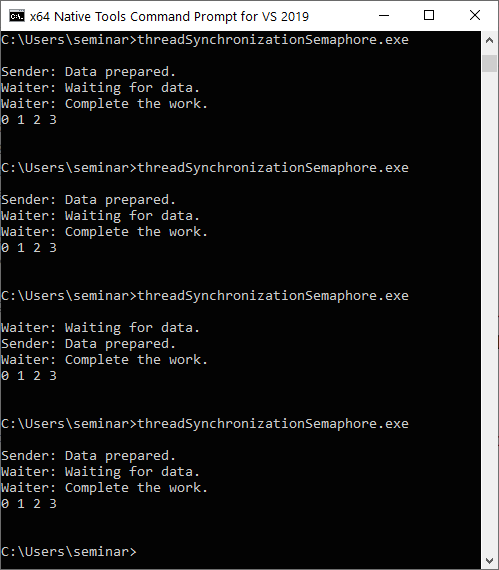
\includegraphics[width=0.6\textwidth]{content/3/chapter6/images/17.png}\\
\end{center}

\begin{tcolorbox}[breakable,enhanced jigsaw,colback=mygreen!5!white,colframe=mygreen!75!black,title={总结}]
	
\begin{itemize}
\item 
信号量是一种同步机制,用于控制对共享资源的并发访问。

\item 
C++20中的计数信号量有一个计数器。获取信号量会减少计数器,释放信号量会增加计数器。若线程试图在计数器为零时获取信号量,则该线程将阻塞,直到另一个线程通过释放信号量来增加计数器。
\end{itemize}
	
\end{tcolorbox}

\newpage
















